A differenza dei casi precedenti, per i $\gamma$ i meccanismi sono totalmente differenti. Ciò perché i $\gamma$, essendo fotoni, sono privi di carica, per cui interagiscono con la materia in maniera diversa.

Nello spettro delle onde elettromagnetiche i raggi $\gamma$ sono le radiazioni più energetiche: corrispondono a energie che vanno da qualche centinaio di keV in su. Poiché nello spettro non c'è una vera e propria distinzione tra la zona dei $\gamma$ e le altre, oltre ai valori di energia bisogna ricordarsi che i fotoni $\gamma$ sono associati a processi legati al nucleo (ad esempio decadimenti $\gamma$ che riguardano le transizioni tra i livelli nucleari, mentre le transizioni tra livelli atomici comportano le emissioni di radiazioni ricadenti nella zona dei raggi $X$). Va ricordato che quanto diciamo riguardo l'interazione dei $\gamma$ è applicabile anche a quella dei raggi $X$.

Oltre le transizioni nucleari, altre sorgenti di raggi $\gamma$ (che peraltro portano a valori di energia più elevati) sono i $\gamma$ presenti nella radiazione cosmica e i $\gamma$ prodotti da collisioni tra fasci di particelle accelerate mediante acceleratori.

\section{Meccanismi di interazione dei fotoni}

I $\gamma$ sono delle radiazioni neutre ed i meccanismi di interazione che caratterizzano questi sono tipicamente catastrofici, nel senso che sono dei processi in cui il $\gamma$ perde una frazione consistente della propria energia, modificando profondamente lo stato iniziale, a differenza delle particelle cariche sia leggere che pesanti in cui l'interazione con la materia avviene gradualmente, attraverso processi multipli di interazione.

I meccanismi attraverso cui i $\gamma$ interagiscono con la materia sono essenzialmente tre:

\begin{itemize}
    \item Effetto fotoelettrico;
    \item Effetto Compton;
    \item Produzione di coppie $e^+ - e^-$.
\end{itemize}

Questa differenza nella modalità di interazione comporta due conseguenze: una prima conseguenza è che i raggi $X$ e $\gamma$ sono radiazioni molto più penetranti rispetto alle particelle cariche; la seconda è che fasci di questi raggi non si degradano in energia quando attraversano la materia, ma solo in intensità. Quindi se un $\gamma$ attraversa la materia ci sono solo due possibilità: o interagisce o non interagisce, per cui non accade, come nel caso delle particelle cariche, che attraversando uno spessore la particella perda parte della sua energia e poi fuoriesca dal materiale, bensì in questo caso o il $\gamma$ interagisce e scompare (perché cambia il suo stato e al suo posto si formano altri prodotti) oppure attraversa il materiale indisturbato; pertanto quando andiamo a studiare l'assorbimento dei $\gamma$ attraverso la materia osserviamo una diminuzione dell'intensità del fascio attraversante lo spessore, ma l'energia dei $\gamma$ fuoriuscenti sarà uguale a quella iniziale. Possiamo dunque dire che i fotoni che conservano il loro stato iniziale sono quelli che non hanno interagito.

A questo punto dobbiamo capire la probabilità con cui avviene ciascuno di questi processi di interazione. In generale si può dire che le sezioni d'urto d'interazione sono molto minori rispetto a quelle relative ai processi con particelle cariche. In altre parole, i fotoni interagiscono molto meno con la materia (ed è per questo che riescono ad attraversare grandi spessori di materiale, cioè hanno un potere penetrante molto più elevato) rispetto alle particelle cariche.

L'attenuazione dei fotoni incidenti in un dato materiale segue una legge di tipo esponenziale decrescente, simile a quella relativa alle particelle cariche leggere (elettroni e positroni), solo che in questo caso è una legge esatta mentre in quel caso era una legge semi-empirica derivante da vari fattori (le particelle non sono monocromatiche, si considera la convoluzione di tante curve di trasmissione ecc.).

L'intensità $I$ del fascio dopo aver attraversato uno spessore $x$ di materiale è data da

\begin{equation*}
    I=I_0 e^{-\mu x}
\end{equation*}

dove $I_0$ è l'intensità iniziale del fascio è $\mu$ è un coefficiente di assorbimento, che esprime la probabilità di interazione dei $\gamma$ per unità di percorso. Si può immaginare come una sorta di inverso del libero cammino medio del fotone all'interno della materia e dipende dal materiale, per cui si misura in $\rm cm^{-1}$ oppure in $\rm cm^2/g$.

Anche in questo caso è possibile possibile realizzare una curva di trasmissione, che ha in ascisse lo spessore attraversato e in ordinate il coefficiente di trasmissione $T=I/I_0$. Quello che otterremmo in questo caso sarebbe un esponenziale decrescente.

Ne approfittiamo per ricordare i vari andamenti:

\begin{itemize}
    \item Per particelle cariche pesanti abbiamo una curva a gradino smussato a causa degli effetti di straggling;
    \item Per particelle cariche leggere, se queste sono mono-energetiche la curva è a gradino ma molto smussato a causa dei percorsi molto frastagliati della particella nel materiale (straggling maggiore), se invece sono $\beta$ emessi da una sorgente, quindi con uno spettro di energia continuo, la curva è approssimabile con una legge esponenziale decrescente;
    \item Per i $\gamma$ la curva è esattamente una legge esponenziale decrescente.
\end{itemize}

Il coefficiente di assorbimento $\mu$ si può esprimere anche nella forma

\begin{equation*}
    \mu=N \sigma_{\rm tot}
    =\frac{N_A \rho}{A} \sigma_{\rm tot}
\end{equation*}

dove si va moltiplicare la sezione d'urto di interazione totale (con cui includiamo tutti i possibili processi di interazione, dunque rappresenta la probabilità di interazione di un fotone con la materia indipendentemente dal tipo di processo) per la densità di atomi $N$. La stessa relazione può essere riscritta con il numero di Avogadro $N_A$, la densità $\rho$ e l'$A$ del materiale. Si evince che maggiore è la probabilità di interazione, maggiore sarà $\mu$, perché significa che il $\gamma$ interagisce di più con la materia e quindi viene più facilmente assorbito.

\subsection{Sezione d'urto di interazione}

La sezione d'urto totale è data dalla somma di quelle relative ai tre processi principali:

\begin{equation*}
    \sigma_{\rm tot}
    =\sigma_{\rm phot} + Z \sigma_{\rm Comp} + \sigma_{\rm coppie}
\end{equation*}

dove la $\sigma_{\rm comp}$ viene moltiplicata per la $Z$ del materiale perché normalmente questa sezione d'urto viene espressa in unità di carica.

Poiché ciascuna di queste componenti è legata ad un processo diverso, esse avranno espressioni dipendenti dalle caratteristiche del materiale e dall'energia del fotone in maniere differenti.

\begin{esempio}
    In figura sono riportate le sezioni d'urto dei singoli processi al variare dell'energia del fotone, la quale va da $\rm 10^{-3} \; MeV (=1 \; keV)$ a $\rm 10^5 \; MeV (=100 \; GeV)$.\footnotemark \;La scala di entrambi gli assi è logaritmica, in modo da poter rappresentare numeri che variano in un intervallo molto ampio, in particolare per la sezione d'urto abbiamo un intervallo di 30 ordini di grandezza.

    \begin{figure}[H]
        \centering
        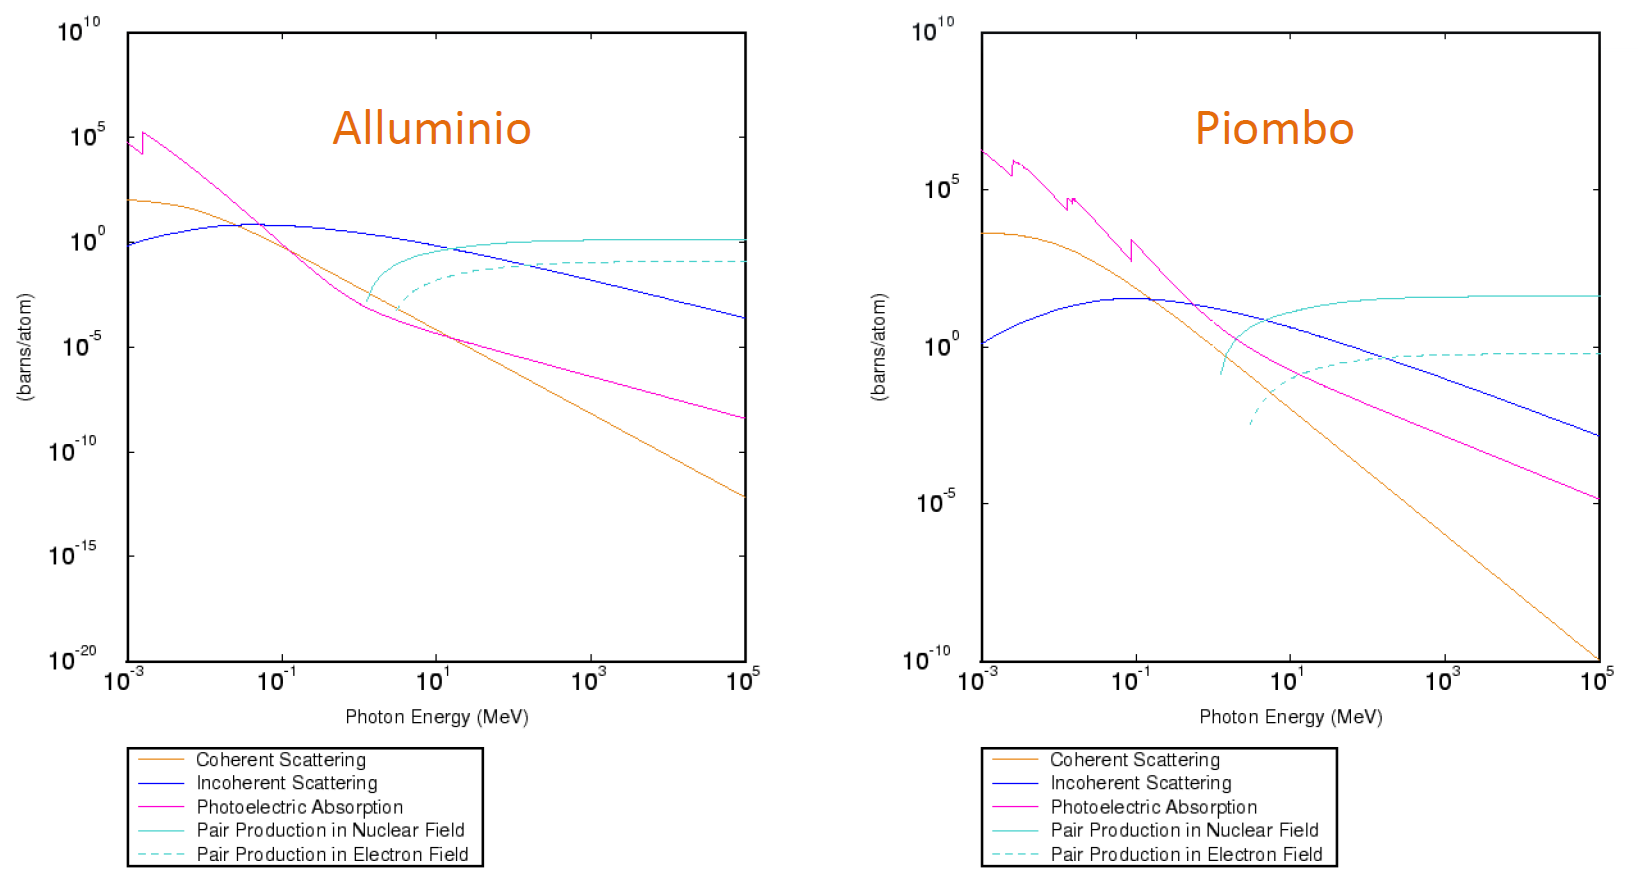
\includegraphics[width=\textwidth]{immagini/sezione_durto_interazione.png}
    \end{figure}
    
    Il contributo dell'effetto fotoelettrico è dato dalla linea fucsia, la quale ci dice che la probabilità che un fotone interagisca per effetto fotoelettrico diminuisce notevolmente all'aumentare dell'energia, per cui per energie più basse domina mentre per quelle più alte (dal GeV in su) è praticamente nulla.

    La linea blu rappresenta lo scattering Compton incoerente, quella arancione quello coerente. Lo scattering coerente si ha quando l'elettrone non fuoriesce dall'atomo, cioè non viene strappato da questo, quello incoerente quando l'elettrone con cui il $\gamma$ interagisce fuoriesce. La curva blu sale per poi scendere, quella arancione non ha salite e diminuisce molto di più. La somma di questi due contributi dà la sezione d'urto dello scattering Compton, che dà una curva che tende leggermente a salire per poi diminuire a più elevate energie ed è una curva che prevale ad energie intermedie.

    Infine le linee azzurre, una continua e una tratteggiata, sono relative al contributo della produzione di coppie. Ce ne sono due perché la produzione di coppie si verifica sempre in presenza di un terzo corpo, che può essere un nucleo o un elettrone, per cui si hanno due casi diversi (la sezione d'urto maggiore è relativa al caso del nucleo). Tale contributo è nullo al di sotto del valore di soglia di 1.022 MeV, dopodiché aumenta fino a diventare il contributo più importante per le energie più elevate.

    Il grafico a sinistra è relativo all'alluminio. Se andiamo a materiali più pesanti come il piombo (grafico a destra) i valori cambiano, ma persistono le considerazioni appena fatte; ciò che invece è più evidente sono le strutture, nella sezione d'urto dell'effetto fotoelettrico, legate alle transizioni atomiche, quindi il valore di energia del fotone che sta incidendo sugli atomi di quel materiale corrisponde esattamente all'energia di una transizione atomica, per cui si vanno a vedere dei picchi.
\end{esempio}

\footnotetext{Per valori che vanno da $10^{-3}$ a $10^{-2}$ MeV si parla di raggi $X$, oltre sono $\gamma$.}

\subsection{Coefficiente di assorbimento}

\begin{esempio}
    In figura è riportato il coefficiente di assorbimento totale per il rame in funzione dell'energia. Esso è riportato in unità di densità superficiale, di modo che le curve ottenute al variare del materiale siano tra loro confrontabili.
    \begin{figure}[H]
        \centering
        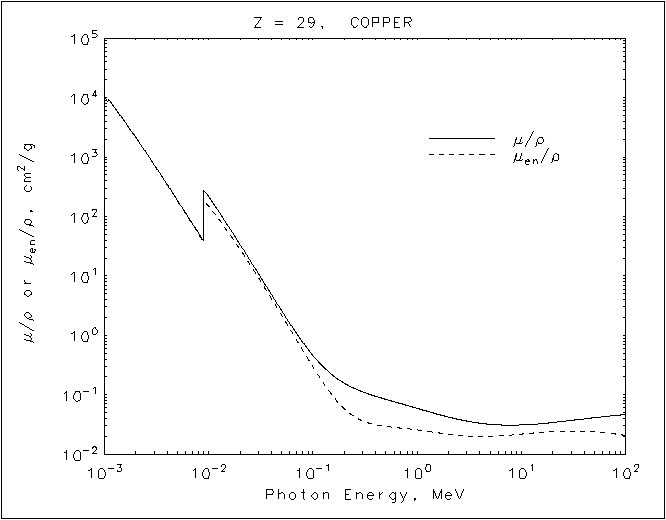
\includegraphics[width=8cm]{immagini/coefficiente_assorbimento_gamma_rame.png}
    \end{figure}
    Per come è definito $\sigma_{\rm tot}$ (ricordiamo che $\mu$ è proporzionale a quest'ultimo), esso avrà un andamento che rispecchia l'andamento della somma delle tre sezioni d'urto. All'aumentare dell'energia $\mu$ diminuisce, per cui se abbiamo dei fotoni di energia molto elevata la probabilità che essi interagiscono con la materia diventa estremamente rara.
    
    Notiamo che nel grafico figurano due linee: la linea continua rappresenta il coefficiente di assorbimento, mentre quella tratteggiata rappresenta il "coefficiente di assorbimento massa-energia", il quale rappresenta la frazione media di particelle cariche prodotte dall'interazione dei gamma con la materia. Infatti tutti e tre i meccanismi di interazione portano alla produzione, nello stato finale, di particelle cariche, e andando a valutare quante ne vengono prodotte si può rappresentare il numero di queste in funzione dell'energia. Ciò che ci aspettiamo è che se i $\gamma$ interagiscono parecchio vengono prodotte tante particelle cariche, dunque anche questo numero è particolarmente elevato; man mano che l'energia aumenta questo numero tende a diminuire perché i $\gamma$ interagiscono di meno. La differenza tra le due curve sta nel fatto che intervengono tutti e tre i processi e ognuno di questi produce un numero di particelle cariche diverso, quindi dipende da qual è l'effetto dominante nella zona di energia in cui ci troviamo.
\end{esempio}

\begin{approfondimento}[Coefficiente di attenuazione e coefficiente di assorbimento]
    \footnotesize Attenzione! Questa nota è stata realizzata unendo quando detto da chatgpt e quanto trovato in "Introduction to Health Physics" di Herman Cember e Thomas E. Johnson. Il lettore attento noterà la discrepanza con quanto affermato dalla professoressa, per cui non garantisco la correttezza delle informazioni riportate.
    
    Approfondiamo il concetto di coefficiente di assorbimento. Diciamo innanzitutto che talvolta nei testi viene chiamato coefficiente di attenuazione, che può essere distinto tra linear attenuation coefficient ($\mu_l$) se espresso in $\rm cm^{-1}$ e mass attenuation coefficient ($\mu_m$) se diviso per la massa e dunque espresso in $\rm cm^2/g$:
    \begin{equation*}
        \mu_{m}=\frac{\mu_l}{\rho}
    \end{equation*}
    Come abbiamo già detto, esso è l'inverso del libero cammino medio. Quest'ultimo il Knoll lo chiama $\lambda$ e lo definisce come
    \begin{equation*}
        \lambda
        =\frac{\int_{0}^{+\infty} xe^{-\mu x} \dd{x}}{\int_{0}^{+\infty} e^{-\mu x} \dd{x}}
        =\frac{1}{\mu}
    \end{equation*}
    Il coefficiente di attenuazione dà la probabilità di rimozione di un fotone dal fascio ad opera di uno dei possibili meccanismi di interazione. Il coefficiente di attenuazione totale, dunque, è dato dalla somma dei coefficienti per ciascuno dei tre processi:
    \begin{equation*}
        \mu=\mu_{\rm phot} + \mu_{\rm Comp} + \mu_{\rm coppie}
    \end{equation*}
    Tale equazione dà la frazione di energia rimossa dal fascio per unità di spessore attraversato. La frazione di energia del fascio che viene depositata nell'assorbitore considera però soltanto l'energia trasferita al materiale dai fotoelettroni, dagli elettroni Compton e dalle coppie $e^+ - e^-$, mentre l'energia trasportata via dal fotone scatterato per effetto Compton e quella portata via dalla radiazione ottenuta per annichilazione di coppie non vengono tenute in conto. Il coefficiente di assorbimento energia, detto anche vero coefficiente di assorbimento, è dato da
    \begin{equation*}
        \mu_{\rm en}
        =\mu_{\rm phot} + \mu_{\rm Comp} + \mu_{\rm coppie} \qty( \frac{h \nu - 1.02}{h\nu} )
    \end{equation*}
    Ovviamente, il coefficiente di assorbimento massa energia si otterrà semplicemente dividendo questo per la densità del materiale.

    \begin{minipage}{0.495\textwidth}
        \begin{figure}[H]
            \centering
            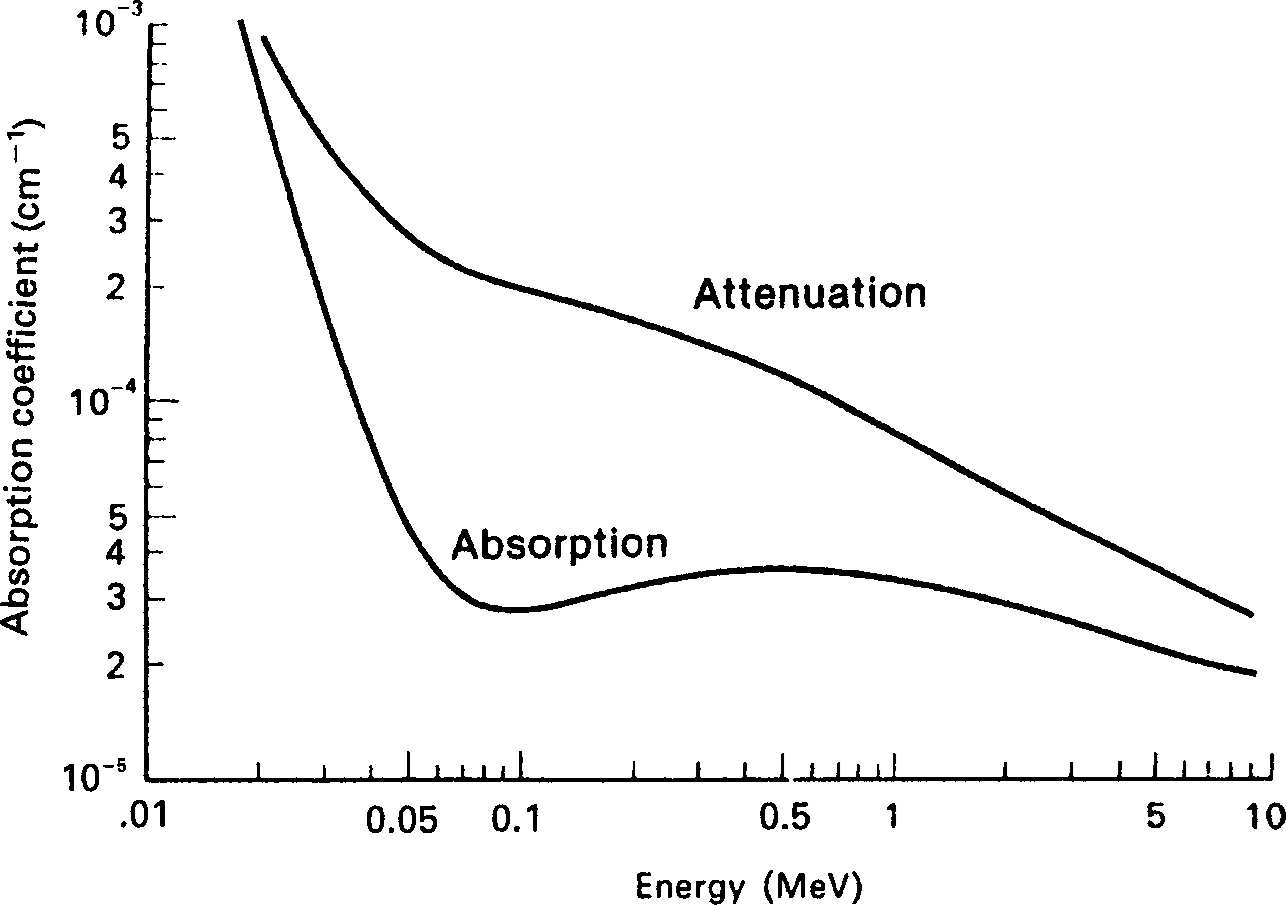
\includegraphics[width=0.8\textwidth]{immagini/coefficiente_assorbimento_vs_attenuazione.png}
        \end{figure}
    \end{minipage}
    \begin{minipage}{0.5\textwidth}
        In sintesi, mentre il coefficiente di assorbimento ($\mu$) riguarda la probabilità di qualsiasi tipo di interazione del fotone gamma con la materia, il coefficiente di assorbimento massa energia ($\mu_{\rm en}$) si focalizza sull'energia effettivamente assorbita e trasferita alla materia, un aspetto cruciale per determinare gli effetti biologici delle radiazioni. In figura a lato possiamo vedere l'andamento dei due termini.
    \end{minipage}

    \vspace{0.2cm}In altri termini ancora, il coefficiente di attenuazione quantifica la riduzione dell'intensità del fascio, mentre il (vero) coefficiente di assorbimento quantifica la frazione di energia assorbita dal fascio, entrambi per unità di spessore di materiale attraversato. Entrambi dipendono dall'energia del fotone e dal materiale.
\end{approfondimento}

Richiamiamo adesso brevemente i tre processi presi in esame.

\subsection{Effetto fotoelettrico}

Esso si verifica solo nel caso di elettroni legati, in quanto un elettrone libero non potrebbe mai assorbire un fotone e assicurare la conservazione dell'impulso, quindi è necessaria la presenza di un nucleo che assorba l'impulso di rinculo.

L'effetto fotoelettrico consiste nel fatto che un fotone (cioè un $\gamma$) venga assorbito totalmente e un elettrone venga emesso dall'atomo, per cui alla fine si ha un elettrone più uno ione:

\begin{figure}[H]
    \centering
    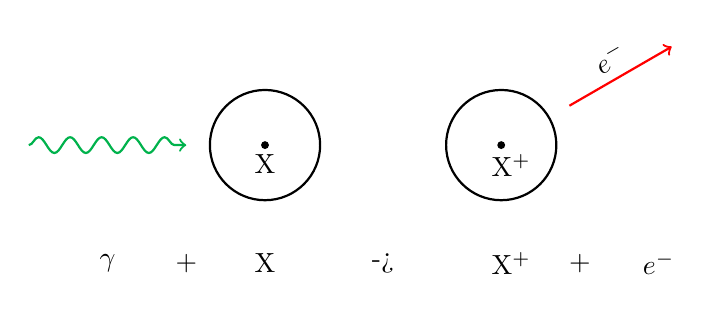
\begin{tikzpicture}
        %figura a sinistra
        \draw[->,thick, teal!60!green, decorate, decoration={snake, segment length=4mm, amplitude=1mm,post length=1mm}] (0,0) -- (2,0);
        \node at (1,-1.5) {$\gamma$};
        \node at (2,-1.5) {$+$};
        \filldraw (3,0) circle (1.2pt) node[below] {X};
        \draw[thick] (3,0) circle (0.7cm);
        \node at (3,-1.5) {X};
        \node at (4.5,-1.5) {\ce{->}};
        %figura a destra
        \draw[->, thick, red,rotate around={30:(6,0)}] (7,0) -- (8.5,0) node[midway, above, rotate=30, black] {$e^-$};
        \filldraw (6,0) circle (1.2pt) node[below] {\hspace{0.25cm}X$^+$};
        \draw[thick] (6,0) circle (0.7cm);
        \node at (6,-1.5) {$\hspace{0.25cm}\rm X^+$};
        \node at (7,-1.5) {$+$};
        \node at (8,-1.5) {$e^-$};
    \end{tikzpicture}
\end{figure}

Affinché ciò avvenga, è necessario che l'energia del fotone incidente superi un certo valore di soglia $W_0$, che è il lavoro di estrazione. In altre parole, il fotone incidente di energia $h\nu$ deve avere un'energia tale da strappare l'elettrone all'atomo, il quale verrà emesso con un'energia cinetica data dalla relazione:

\begin{equation*}
    K_{\rm max}=h\nu - W_0
\end{equation*}

$W_0$ è dell'ordine di pochi eV ma dipende dal materiale.

Essendo i $\gamma$ fotoni ad altissima energia siamo certamente al di sopra del lavoro di estrazione degli elettroni di un qualsiasi materiale, inoltre in questo caso possiamo dire che l'energia cinetica $K_{\rm max}$ dell'elettrone espulso dall'atomo può essere approssimata all'energia del fotone incidente\footnote{Infatti per dare un'idea delle quantità in gioco possiamo immaginare di avere un $\gamma$ di energia 1 MeV che incide su un materiale avente lavoro di estrazione pari a 2 eV: il fotoelettrone emesso avrà energia pari a $(10^6 - 2)$ eV, che è una differenza irrisoria.}. Di conseguenza, nel caso delle sorgenti $\gamma$ che adopereremo in laboratorio varrà questa approssimazione, cioè potremo dire che gli elettroni emessi per effetto fotoelettrico hanno energia praticamente identica a quella del $\gamma$ incidente.

Ribadiamo che non sempre è così: se andiamo verso radiazioni a più basse energie la differenza non è più trascurabile, seppur si riesca comunque a produrre effetto fotoelettrico (ad esempio la luce visibile può produrre effetto fotoelettrico su alcuni materiali, così come vedremo utilizzando dei led per misurare la costante di Planck).

\begin{minipage}{0.395\textwidth}
    \begin{figure}[H]
        \centering
        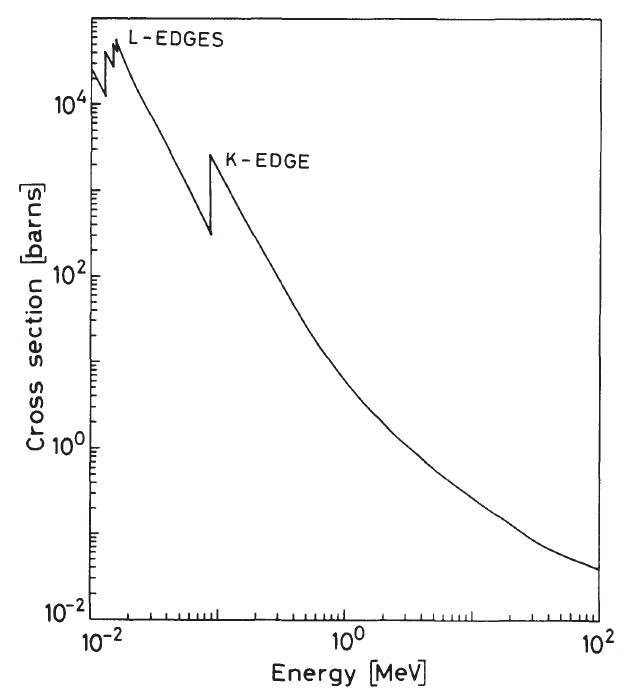
\includegraphics[width=0.9\textwidth]{immagini/sezione_durto_effetto_fotoelettrico.png}
    \end{figure}
\end{minipage}
\begin{minipage}{0.6\textwidth}
    La sezione d'urto per effetto fotoelettrico dipende dal materiale e dall'energia della radiazione $\gamma$ incidente mediante una relazione del tipo

    \begin{equation*}
        \sigma_{\rm phot} \approx \frac{Z^5}{E_{\gamma}^{7/2}}
    \end{equation*}

    Ne segue che per agevolare l'effetto fotoelettrico conviene considerare materiali via via più pesanti, a $Z$ maggiore, mentre la dipendenza dall'energia del $\gamma$ spiega la brusca diminuzione di $\sigma$ vista nei grafici.
\end{minipage}

\vspace{0.3cm}In realtà tale dipendenza da $Z$ è valida solo per un certo intervallo di energie. Ad esempio a basse energie viene modificata. Il motivo è che valutare la sezione d'urto di questo processo non è semplice a causa della complessità delle funzioni d'onda degli elettroni negli atomi. Questa dipendenza dunque si presenta per energie al di sopra della shell K (livello 1s), a circa $10^{-1}$ MeV, per valori più bassi cambia forma\footnote{Ti aspettavi un approfondimento a questo punto? Non stavolta! Servono concetti di AQM e qui siamo solo alla triennale, non bruciamo le tappe.}.

Nella figura sopra possiamo vedere l'andamento della sezione d'urto per effetto fotoelettrico nel caso del piombo. Notiamo come la parte iniziale è caratterizzata dalle transizioni atomiche. Ricordiamo che esso governa l'interazione a basse energie.

\subsection{Effetto Compton}

\E un effetto di scattering di un fotone su un elettrone.

\begin{figure}[H]
    \centering
    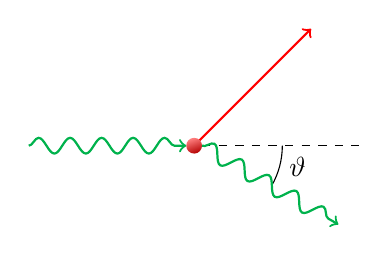
\begin{tikzpicture}
        %elettrone
        \draw[thick,->,red,rotate around={45:(2.1,0)}] (2.1,0) -- (4.2,0); 
        \shade[top color=red!50,bottom color=red!70!black,shading angle=20] (2.1,0) circle (0.1cm);
        %fotone incidente
        \draw[->,thick, teal!60!green, decorate, decoration={snake, segment length=4mm, amplitude=1mm,post length=1mm}] (0,0) -- (2,0);
        %angolo
        \draw[dashed] (2.2,0) -- (4.2,0);
        \draw (3.22,0) arc (0:-30:1.02cm) node[midway, right] {$\vartheta$};
        %fotone riflesso
        \draw[->,thick, teal!60!green, decorate, decoration={snake, segment length=4mm, amplitude=1mm,post length=1mm},rotate around={-30:(2.2,0)}] (2.2,0) -- (4.2,0);
      \end{tikzpicture}
\end{figure}

In questo caso si considera l'effetto su un elettrone libero. In realtà gli elettroni sono quelli atomici, però si può considerare un elettrone atomico come libero per il fatto che le energie di legame degli elettroni sono normalmente molto più piccole rispetto alle energie dei $\gamma$ considerati, quindi è un'approssimazione lecita. 

A seguito dello scattering, nello stato finale avremo un fotone diffuso, con energia $h\nu'$ inferiore rispetto all'energia $h\nu$ del fotone incidente, e un elettrone.

Indicando con $\vartheta$ l'angolo di diffusione del fotone uscente, applicando la conservazione dell'energia e dell'impulso è possibile individuare una relazione che lega l'energia del fotone diffuso con l'angolo:
\begin{equation*}
    h\nu'=\frac{h\nu}{\big[1 + \gamma (1 - \cos{\vartheta})\big]}
    \qqtext{dove}
    \gamma=\frac{h\nu}{m_ec^2}
\end{equation*}
Quindi in base al valore di $\vartheta$, che varia da evento a evento, le energie ripartite tra l'elettrone e il fotone diffuso possono essere differenti.
Per la conservazione dell'energia, l'energia cinetica dell'elettrone sarà data dalla differenza tra l'energia del fotone incidente e quello diffuso:
\begin{equation*}
    T_e=h\nu - h\nu'
\end{equation*}
Tale processo domina a energie intermedie.

Lo scattering Compton si definisce coerente quando l'elettrone, che consideriamo libero ma in realtà non lo è, rimane legato all'atomo; se invece l'elettrone acquisisce un'energia tale da poter essere strappato dall'atomo si parla di scattering incoerente. Più precisamente:

\begin{itemize}[leftmargin=0.5cm]
    \item Lo scattering coerente (anche noto come scattering di Rayleigh) si verifica quando il fotone è deviato dalla sua traiettoria originale senza perdita di energia. In questo caso, l'interazione è elastica e avviene principalmente con l'intero atomo piuttosto che con singoli elettroni. Anche se lo scattering coerente non modifica l'energia del fotone, può comunque contribuire alla diffusione della radiazione;
    \item Lo scattering incoerente, che si riferisce specificamente allo scattering Compton, si verifica quando il fotone cede parte della sua energia a un elettrone e viene diffuso con una lunghezza d'onda maggiore. Questa interazione è inelastica e comporta un cambiamento nella lunghezza d'onda del fotone.
\end{itemize}

La sezione d'urto Compton è data da due termini che corrispondono a quello coerente e a quello incoerente\footnote{Questa affermazione è parzialmente in contrasto con quanto detto subito dopo. Non è sbagliato dire che i due contributi sono questi, ma quelli mostrati nel grafico sono altri due.}. Si osserva una dipendenza lineare da $Z$, e una diminuzione che ad alte energie può essere parametrizzata con una dipendenza del tipo $(\ln E)/E$.

\begin{minipage}{0.375\textwidth}
    \begin{figure}[H]
        \centering
        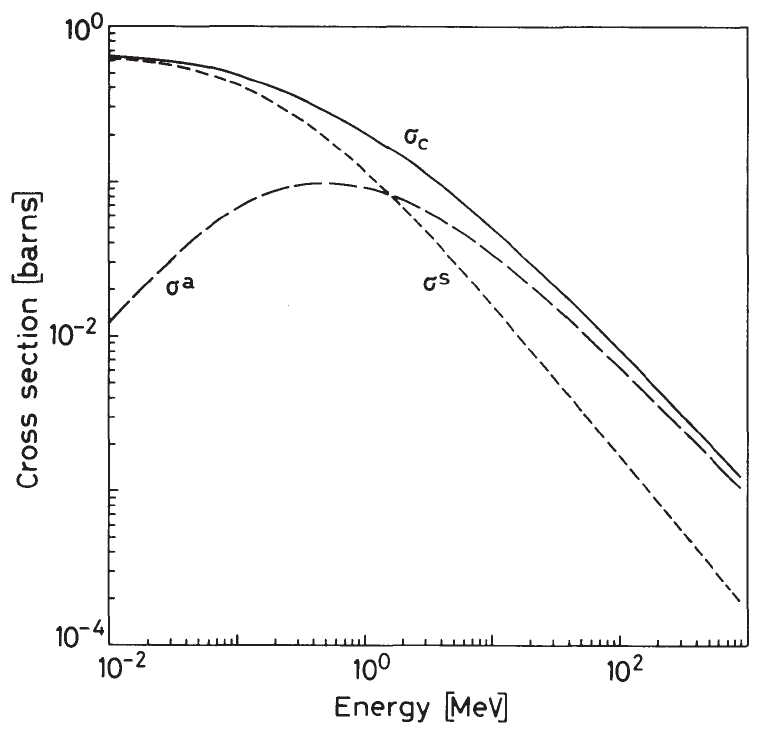
\includegraphics[width=\textwidth]{immagini/sezione_durto_effetto_Compton.png}
    \end{figure}
\end{minipage}
\begin{minipage}{0.62\textwidth}
    Due quantità utili che possono essere calcolate tramite la formulazione di Klein-Nishina sono le sezioni d'urto di scattering Compton e di assorbimento Compton. La sezione d'urto di scattering Compton, $\sigma_{\rm s}$, è definita come la frazione media dell'energia totale contenuta nel fotone diffuso, mentre la sezione d'urto di assorbimento, $\sigma_{\rm a}$, è l'energia media trasferita all'elettrone di rinculo. Poiché l'elettrone è fermato dal materiale, questa è la frazione media di energia assorbita dal materiale nello scattering Compton. Ovviamente si ha
\end{minipage}

\begin{equation*}
    \sigma_{\rm Comp}=\sigma_{\rm a} + \sigma_{\rm s}
\end{equation*}

Attenzione! Rispetto ai grafici precedenti in questo sembra che tale contributo decresca più velocemente, ma ciò è dovuto semplicemente al fatto che stiamo considerando un intervallo più ristretto di energie.

\subsection{Creazione di coppie}

Con questo processo si ha una creazione di una coppia elettrone-positrone a partire da un $\gamma$. Ciò può avvenire solo in presenza di un terzo corpo per questioni di conservazione dell'impulso.

\begin{figure}[H]
    \centering
    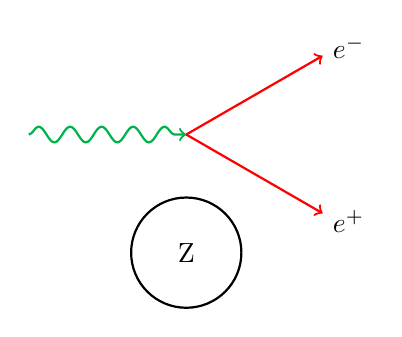
\begin{tikzpicture}
        \draw[thick,->,red,rotate around={30:(2,0)}] (2,0) -- (4,0) node[above=.1cm, right, black] {$e^-$};
        \draw[thick,->,red,rotate around={-30:(2,0)}] (2,0) -- (4,0) node[below=.1cm, right, black] {$e^+$};
        %fotone incidente
        \draw[->,thick, teal!60!green, decorate, decoration={snake, segment length=4mm, amplitude=1mm,post length=1mm}] (0,0) -- (2,0);
        \draw[thick] (2,-1.5) node {Z} circle (0.7cm);
      \end{tikzpicture}
\end{figure}

Questo terzo corpo tipicamente è il nucleo atomico, ma alcune volte tale processo può avvenire anche nel campo degli elettroni, infatti nel grafico della sezione d'urto c'erano due termini relativi alla produzione di coppie, ma quello relativo al caso dell'elettrone è trascurabile rispetto all'altro.

La coppia prodotta deve rispettare la conservazione dell'energia, per cui l'energia cinetica delle due particelle uscenti corrisponde all'energia del fotone incidente meno due volte la massa a riposo dell'elettrone:

\begin{equation*}
    T(e^+) + T(e^-)=h\nu - 2mc^2
\end{equation*}

Ciò ha senso, perché parte dell'energia del fotone deve essere usata per la produzione delle due masse.

\begin{minipage}{0.395\textwidth}
    \begin{figure}[H]
        \centering
        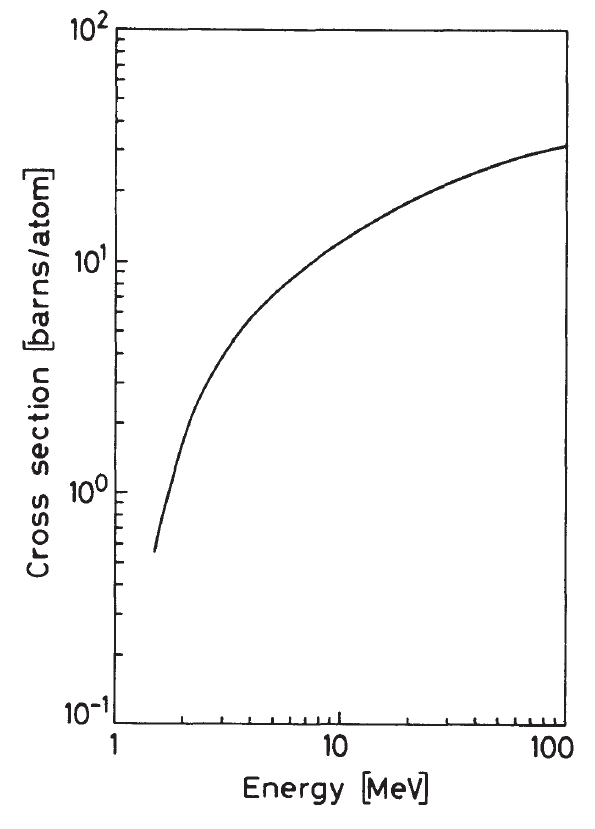
\includegraphics[width=5cm]{immagini/sezione_durto_produzione_coppie.png}
    \end{figure}
\end{minipage}
\begin{minipage}{0.6\textwidth}
    Da tale relazione segue che ci sia una soglia di produzione al di sotto della quale è impossibile che si verifichi il processo di produzione di coppie. Quindi, se il fotone incidente non ha un'energia sufficiente almeno a creare questa coppia (cioè almeno $2mc^2=1.022$ MeV), non avviene nessun processo; se ha un'energia superiore alla soglia, quella in eccesso viene poi suddivisa tra i prodotti, cioè tra elettrone e positrone.

    La sezione d'urto è proporzionale a $Z^2$ e cresce con l'energia, infatti è il processo che domina ad energie elevate.
\end{minipage}

\vspace{0.2cm}In figura possiamo vedere l'andamento della sezione d'urto per produzione di coppie in funzione dell'energia nel caso del piombo. Notiamo come essa sia nulla al di sotto del valore di soglia.

\subsection{Sommario}

\begin{itemize}
    \item A basse energie (ordine del MeV) i fotoni interagiscono prevalentemente mediante effetto fotoelettrico, che produce un elettrone avente pressoché la stessa energia del $\gamma$;

    \item Per energie tra 1 e 10 MeV prevale l'effetto Compton, che produce un elettrone ed un fotone diffuso che si dividono l'energia del fotone iniziale;
    \item Ad alte energie (sopra i 10 MeV) prevale il processo di produzione di coppie, che nello stato finale produce una coppia $e^+ - e^-$.
\end{itemize}

\section{Sciami elettromagnetici}

Ci chiediamo adesso come interagiscono questi prodotti secondari (elettroni, positroni, fotoni) con la materia. Infatti, se in partenza abbiamo elettroni o fotoni di energia particolarmente elevata, si innesca un meccanismo di produzione a valanga, nel senso che si produce una \textit{cascata elettromagnetica} (o sciame e.m.), che è una sequenza di processi di bremsstrahlung e di produzione di coppie che porta alla produzione di un insieme di particelle ($e^+, e^-$, fotoni) che man mano si propagano nella materia.

\begin{figure}[H]
    \centering
    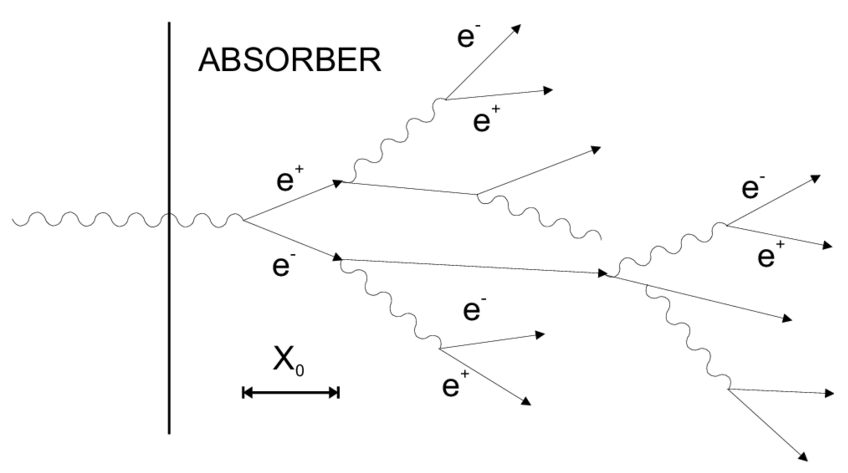
\includegraphics[width=0.75\textwidth]{immagini/sciame_elettromagnetico.png}
\end{figure}

Immaginiamo ad esempio di avere inizialmente un fotone particolarmente energetico che incide su un materiale assorbitore. Avendo energia elevata, ad un certo punto darà luogo ad un processo di produzione di coppie $e^+ - e^-$. Ciascuna di queste sarà ad alta energia, per cui perderà una parte della propria energia attraverso bremsstrahlung, quindi la sequenza continua con un fotone di bremsstrahlung e il positrone/elettrone di partenza che a loro volta daranno luogo ad altri processi che saranno produzioni di coppie o ulteriori processi di bremsstrahlung. Da un singolo fotone incidente di alta energia si produce quindi uno sciame elettromagnetico, composto da un numero di particelle via via crescente.

Uno sciame elettromagnetico può essere indotto, oltre che da un fotone ad alta energia, anche da un elettrone o un positrone ad alta energia, solo che in questo caso il primo processo sarà di bremsstrahlung e non di produzione di copie. Essi vengono detti elettromagnetici perché sono sciami in cui vengono coinvolti solo processi elettromagnetici. Sono composti da $e^+,e^-$ e $\gamma$ (fotoni) e si differenziano dagli sciami adronici, che sono indotti da adroni ad alta energia (ad esempio un protone ad alta energia prodotto in una collisione nucleare) e in cui vi sono processi che coinvolgono l'interazione forte. Tuttavia tali sciami potrebbero avere al loro interno anche una componente elettromagnetica, legata alla possibile produzione di pioni neutri $\pi^0$, i quali decadono in due $\gamma$ che poi daranno luogo a processi elettromagnetici e dunque a questa componente.

Man mano che lo sciame si propaga all'interno del materiale continuano a verificarsi in successione processi di bremsstrahlung e produzione di coppie; questo meccanismo però non procede all'infinito, perché man mano le energie dei prodotti secondari diminuiscono, in quanto l'energia iniziale si suddividerà tra un numero di particelle via via crescente, fin quando l'energia degli elettroni/positroni arriverà al di sotto del valore di energia critica (energia in corrispondenza della quale la sezione d'urto per perdita di energia collisionale è uguale a quella per perdita di energia radiativa, dunque la probabilità dei due processi è la stessa). Quando gli elettroni raggiungono tale valore, non interagiscono con la materia soltanto attraverso fenomeni di bremsstrahlung ma possono subire anche fenomeni collisionali, in cui non vengono prodotte nuove particelle.

Per quanto riguarda i fotoni, man mano che la loro energia diminuisce non daranno luogo a produzioni di coppie, ma cominceranno a prevalere altri effetti che non aumentano il numero di particelle, come quello fotoelettrico (che da un fotone ci dà un elettrone) e quello Compton\footnote{Il lettore attento ricorderà che parlando dello scattering Compton incoerente abbiamo detto che con questo viene strappato un elettrone dall'atomo, quindi in linea teorica con tale fenomeno il numero di particelle dovrebbe comunque aumentare. Bisogna però considerare che quello che stiamo presentando è un modello molto semplificato, mentre stime più esatte si fanno attraverso delle simulazioni numeriche; inoltre man mano si va ad energie sempre più basse, dove prevale l'effetto fotoelettrico. Sebbene quindi non sia del tutto corretto dire che non vengano prodotte nuove particelle proprio dall'energia critica in poi, questa approssimazione ci permette di ottenere delle relazioni che sono abbastanza realistiche.} (che dà un fotone diffuso). In conseguenza a ciò, sebbene non possiamo dire che lo sciame si arresti perché le particelle continueranno a propagarsi all'interno del materiale finché non perdono tutta la loro energia, possiamo dire che il numero di particelle dello sciame non aumenterà superato il punto critico.

Al di sotto dell'energia critica possiamo quindi immaginare che lo sciame che man mano è cresciuto (sia in dimensioni che nel numero di particelle), incomincia a degradarsi, pertanto il numero di particelle comincia a diminuire perché esse continuano a interagire, perdendo energia e venendo assorbite totalmente dal materiale.

\subsection{Struttura di uno sciame elettromagnetico (toy model)}

Proviamo ora a immaginare un modello semplificato per descrivere la struttura di uno sciame elettromagnetico.

Esso si basa sul concetto di lunghezza di radiazione, in quanto la distanza percorsa viene espressa in multipli di questa. Immaginiamo infatti che in corrispondenza di ogni lunghezza di radiazione si verifichi in media un nuovo processo che può essere di produzione di coppie o di bremsstrahlung. Si definisce quindi il \textit{numero di generazione} $t$, dato al rapporto tra lo spazio percorso e la lunghezza di radiazione:

\begin{equation*}
    t=\frac{x}{x_0}
\end{equation*}

Banalmente, esso ci darà il numero di lunghezze di radiazione percorse.

Guardiamo adesso il seguente schema:

%\newpage

\begin{figure}[H]
    \centering
    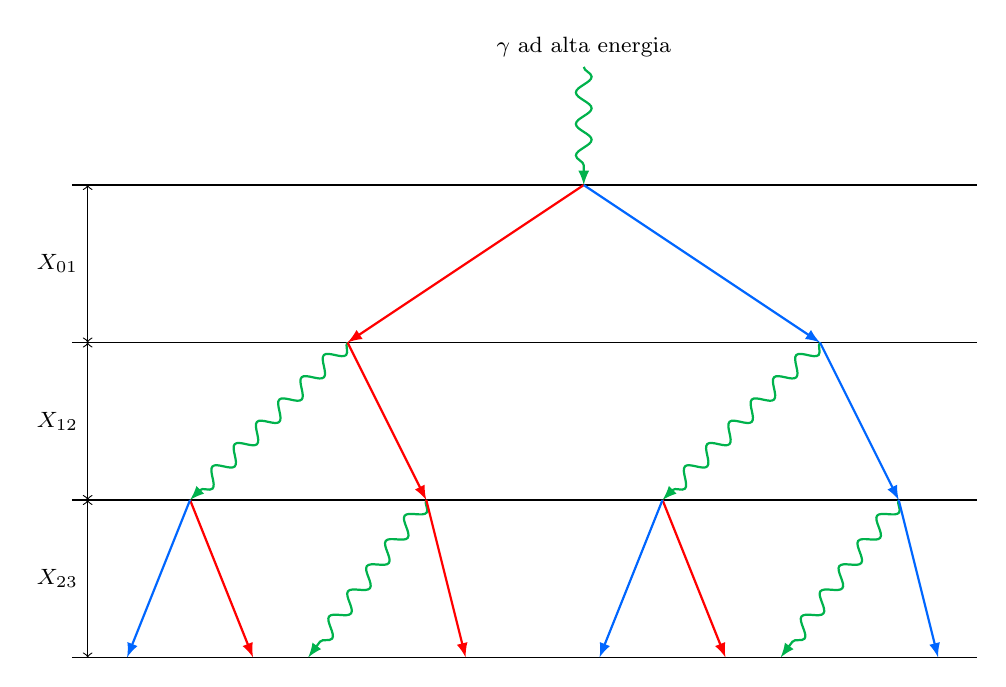
\begin{tikzpicture}
        %livello 0
        \draw (-6.5,0) -- (5,0);
        \draw[-latex,thick, teal!60!green, decorate, decoration={snake, segment length=4mm, amplitude=1mm,post length=1mm}] (0,1.5) node[above,black] {\footnotesize $\gamma$ ad alta energia} -- (0,0);
        %livello 1
        \draw (-6.5,-2) -- (5,-2);
        \draw[thick,red,-latex] (0,0) -- (-3,-2);
        \draw[thick,blue!60!cyan,-latex] (0,0) -- (3,-2);
        %livello 2
        \draw (-6.5,-4) -- (5,-4);
          %sinistra
        \draw[-latex,thick, teal!60!green, decorate, decoration={snake, segment length=4mm, amplitude=1mm,post length=1mm}] (-3,-2) -- (-5,-4);
        \draw[thick,red,-latex] (-3,-2) -- (-2,-4);
          %destra
        \draw[-latex,thick, teal!60!green, decorate, decoration={snake, segment length=4mm, amplitude=1mm,post length=1mm}] (3,-2) -- (1,-4);
        \draw[thick,blue!60!cyan,-latex] (3,-2) -- (4,-4);
        %livello 3
        \draw (-6.5,-6) -- (5,-6);
          %sinistra
        \draw[thick,red,-latex] (-5,-4) -- (-4.2,-6);
        \draw[thick,blue!60!cyan,-latex] (-5,-4) -- (-5.8,-6);
          %centro sinistra
        \draw[-latex,thick, teal!60!green, decorate, decoration={snake, segment length=4mm, amplitude=1mm,post length=1mm}] (-2,-4) -- (-3.5,-6);
        \draw[thick,red,-latex] (-2,-4) -- (-1.5,-6);
          %centro destra
        \draw[thick,red,-latex] (1,-4) -- (1.8,-6);
        \draw[thick,blue!60!cyan,-latex] (1,-4) -- (0.2,-6);
          %destra
          \draw[-latex,thick, teal!60!green, decorate, decoration={snake, segment length=4mm, amplitude=1mm,post length=1mm}] (4,-4) -- (2.5,-6);
          \draw[thick,blue!60!cyan,-latex] (4,-4) -- (4.5,-6);
        %lunghezze di radiazione
        \draw[<->] (-6.3,0) -- (-6.3,-2) node[midway,left] {\footnotesize $X_{01}$};
        \draw[<->] (-6.3,-2) -- (-6.3,-4) node[midway,left] {\footnotesize $X_{12}$};
        \draw[<->] (-6.3,-4) -- (-6.3,-6) node[midway,left] {\footnotesize $X_{23}$};
      \end{tikzpicture}
\end{figure}

In questo esempio abbiamo in partenza un $\gamma$ di alta energia che interagisce, producendo quindi una coppia $e^+ - e^-$; questa coppia percorre uno spazio pari all'incirca ad una lunghezza di radiazione e poi dà luogo a bremsstrahlung, con cui viene prodotto un fotone e un elettrone/positrone come stato finale. Dopo un'altra lunghezza di radiazione il fotone produrrà una coppia mentre l'elettrone e il positrone produrranno bremsstrahlung.

\subsection{Profondità di uno sciame e.m.}

Notiamo come, indipendentemente dal tipo di particella che consideriamo, ogni volta che si percorre uno spazio pari ad una lunghezza di radiazione quello che succede è che ogni particella si raddoppia. Possiamo generalizzare questo meccanismo affermando che il numero $n$ di particelle prodotte dopo $t$ lunghezze di radiazione sarà pari a
\begin{equation*}
    n(t)=2^t
\end{equation*}
Ad esempio, per $t=3$ dovremmo avere 8 particelle, come vediamo effettivamente in figura.

Quale sarà l'energia di queste particelle? Come abbiamo detto, man mano l'energia si degrada perché l'energia del fotone incidente viene via via suddivisa nei prodotti di questa cascata; possiamo allora dire che le particelle della $t$-esima generazione avranno in media energia $E(t)$ pari all'energia $E_0$ del fotone incidente divisa per $n(t)$. In formule:
\begin{equation*}
    E(t)=\frac{E_0}{2^t}
\end{equation*}
A partire da questa relazione possiamo andare a valutare quante particelle vengono prodotte in corrispondenza dell'energia critica, che possiamo immaginare come il valore per cui si ha il massimo dello sciame, inteso come il massimo numero delle particelle dello sciame. In particolare, quando l'energia media delle particelle diviene uguale all'energia critica $E_c$, cioè quando
\begin{equation*}
    \frac{E}{2^t}=E_c
\end{equation*}
non verranno più prodotte nuove particelle e lo sciame non si sviluppa ulteriormente. Per determinare lo spazio che ha percorso lo sciame fino a raggiungere questa condizione basterà valutare quante lunghezze di radiazione sono state percorse, e per fare ciò basta ricavare da questa equazione il valore di $t$ con semplici passaggi:
\begin{equation*}
    \frac{E_0}{2^t}=E_c
    \implies
    \frac{E_0}{E_c}=2^t
    \implies
    t=\frac{\ln{(E_0/E_c)}}{\ln{2}}
\end{equation*}
Da ciò si evince come il punto in cui si raggiunge il numero massimo di particelle dipende con una relazione logaritmica dall'energia incidente $E_0$, ovvero dall'energia del fotone o dell'elettrone iniziale.

\begin{esempio}[Le dimensioni di un calorimetro]
    La relazione appena vista ci permette di determinare lo spessore di un dato materiale necessario per poter contenere o addirittura arrestare lo sciame di una data energia. Ciò è importante dal punto di vista della rivelazione, perché esistono dei rivelatori che prendono il nome di calorimetri, i quali sono dei rivelatori progettati per misurare tutta l'energia di una particella incidente; se quindi ad esempio volessimo misurare l'energia di $\gamma$ o elettroni molto energetici mediante calorimetri, siccome quello che succederà quando questo $\gamma$ o questo elettrone entra nel rivelatore sarà la produzione di uno sciame (perché questo è quello che avviene in qualsiasi materiale), allora per misurare tutta l'energia dello sciame dobbiamo assicurarci che tutte le particelle prodotte nello sciame rimangano all'interno del rivelatore, pertanto il rivelatore non può essere troppo corto perché quello che altrimenti potrebbe succedere è che lo sciame comincia a propagarsi ma poi fuoriesce dal materiale e dunque perdiamo parte dello sciame e di conseguenza parte dell'energia. \E quindi fondamentale che la dimensione del rivelatore sia adeguata a quella dello sciame che può formarsi. Vediamo allora degli esempi numerici.

    Ci chiediamo che spessore debba avere un calorimetro per poter misurare tutta l'energia di un $\gamma$ avente inizialmente un'energia $E_0=10E_c$. Dalla relazione appena vista possiamo calcolare il numero di lunghezze di radiazione:
    \begin{equation*}
        t=\frac{\ln (10E_c/E_c)}{\ln 2}=\frac{\ln 10}{\ln 2}=3.3
    \end{equation*}
    Dunque operando un rivelatore di dimensioni pari a $3,3X_0$ siamo sicuri che catturiamo almeno il massimo sviluppo dello sciame, quindi lo sciame arriva a propagarsi fino al suo massimo sviluppo\footnotemark.

    Se invece l'energia del fotone o dell'elettrone incidente è pari a $100E_c$, il massimo si raggiungerà per
    \begin{equation*}
        t=\frac{\ln (100E_c/E_c)}{\ln 2}=\frac{\ln 100}{\ln 2}=6.6
    \end{equation*}
    Notiamo come, a causa della dipendenza logaritmica dall'energia, nonostante l'energia iniziale sia aumentata di un fattore 10 rispetto al caso precedente lo spessore necessario è soltanto raddoppiato. Ciò costituisce un vantaggio dal punto di vista pratico, perché è possibile realizzare dei calorimetri tutto sommato compatti in grado comunque di misurare buona parte dello sciame anche per $\gamma$ o elettroni di elevata energia.
\end{esempio}

\footnotetext{In realtà vedremo in seguito che sarà necessario considerare spessori maggiori, perché lo sciame una volta raggiunta l'energia critica non si arresta bensì continua a proseguire.}

Bisogna inoltre considerare che siccome il risultato è espresso in multipli di lunghezza di radiazione, la lunghezza vera e propria dipenderà dal tipo di materiale attraversato, in quanto la lunghezza di radiazione dipende dallo $Z$ del materiale; ad esempio, in base ai valori della tabella vista in \S\ref{par:lunghezza_di_radiazione}, affinché venga contenuto fino al massimo uno sciame avente energia iniziale pari $E_0=10E_c$ un rivelatore costruito in piombo dovrà essere lungo $1,8$ cm, mentre se come materiale assorbitore considerassimo l'acqua sarebbero necessari $1,18$ m. %Il fatto che esprimiamo tale variabile in termini di multipli di lunghezza di radiazione ci permette però di essere in qualche modo indipendenti dal tipo di materiale che si sta adoperando.

\subsection{Numero di particelle in uno sciame e.m.}

Guardiamo adesso un altro aspetto dello sciame elettromagnetico, in particolare andiamo a vedere il numero di fotoni e elettroni prodotti in uno sciame in funzione della profondità. Abbiamo infatti intuito che effettivamente si arriva a un massimo nel numero di particelle prodotte, però ancora non abbiamo visto cosa succede dopo questo perché il modello che abbiamo considerato prima era un modello semplificato che non dice nulla su ciò che avviene dopo, in quanto assume che una volta raggiunto il massimo del numero di particelle è come se lo sciame si bloccasse bruscamente, ma in realtà non è così: sappiamo che sono state formate un numero di particelle ($e^+$, $e^-$ e $\gamma$) che proseguiranno attraverso altri meccanismi, venendo man mano assorbite.

Se allora vogliamo vedere l'evoluzione nel numero di fotoni e elettroni in funzione della distanza percorsa non basta quel modello semplificato, ma in realtà sono necessari delle simulazioni numeriche un po' più complesse. Guardiamo il seguente grafico:

\begin{figure}[H]
    \centering
    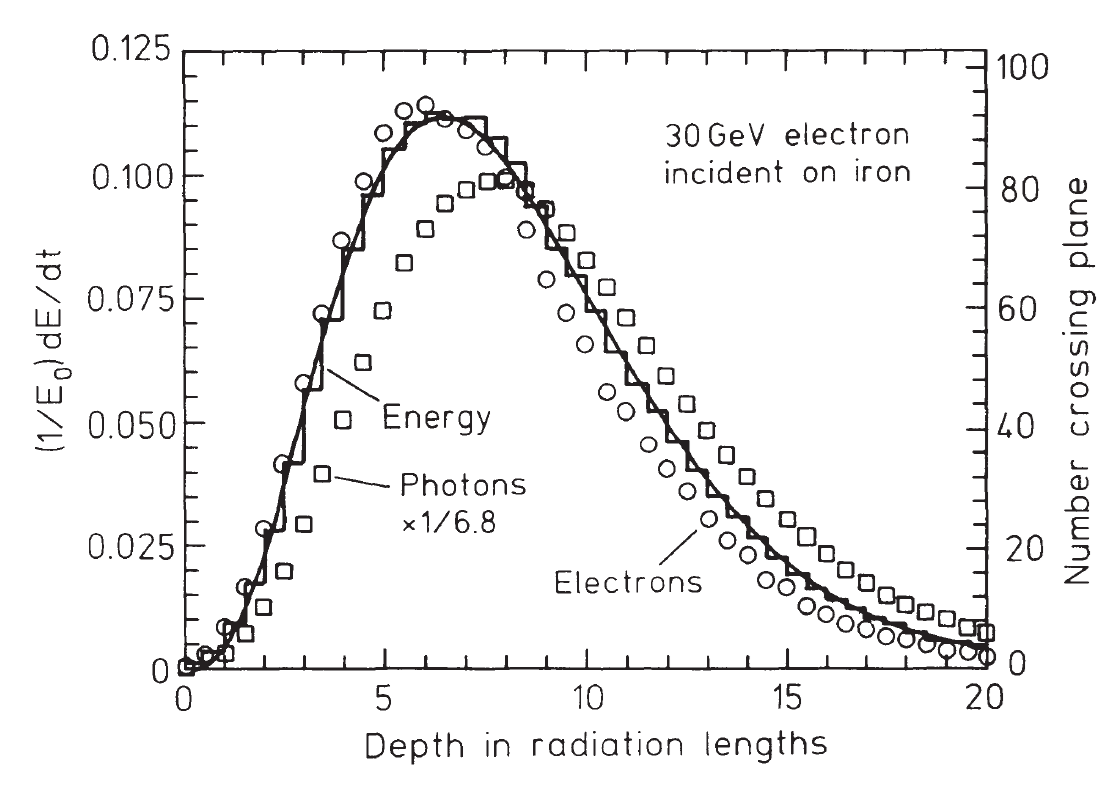
\includegraphics[width=0.6\textwidth]{immagini/numero_particelle_sciame_elettromagnetico.png}
\end{figure}

In tale grafico, realizzato mediante simulazioni Monte Carlo, sull'asse delle ascisse è riportata la distanza percorsa in multipli di lunghezze di radiazione e sull'asse delle ordinate vediamo da un lato la perdita di energia (quindi quanta energia viene persa dallo sciame man mano che si propaga), rappresentata dall'istogramma, e dall'altro il numero di elettroni e fotoni\footnote{In realtà i fotoni sono stati scalati per un fattore $1/6,8$ in modo da rappresentarli in unico grafico assieme agli elettroni, quindi in realtà il numero di questi è molto più grande.}, rappresentati dai pallini e i quadretti.

Guardando l'andamento di questi punti ci rendiamo conto che l'andamento iniziale coincide con quello che ci aspettavamo, ovvero che man mano che lo sciame si propaga all'interno del materiale si ha una crescita praticamente esponenziale nel numero di particelle dettata dalla relazione vista prima; man mano si raggiungerà un massimo, in corrispondenza del quale cominciano a intervenire gli altri meccanismi di interazione. Lo sciame però non si arresta qui: continuerà a propagarsi anche per uno spazio notevole (ad esempio nel grafico per 20 lunghezze di radiazione) e via via il numero di elettroni e di fotoni diminuirà fino ad arrivare ad un punto in cui tutti gli elettroni e tutti i fotoni saranno totalmente assorbiti dal materiale.

Capiamo quindi che è necessario adoperare un materiale sufficientemente lungo per poter contenere tutto lo sciame, in quanto se in termini di lunghezza ci fermassimo semplicemente al massimo andremmo a perdere tutte le altre particelle che continuano a proseguire nel materiale e che perdono energia. In altre parole, se volessimo ricostruire l'energia del $\gamma$ o dell'elettrone incidente e ci limitassimo a utilizzare un materiale che contiene solamente una parte dello sciame, ad esempio fino al suo sviluppo massimo, perderemmo tutto il contributo delle particelle che proseguono nel loro percorso.

\subsection{Sviluppo longitudinale di uno sciame e.m.}

Quando si analizza uno sciame, lo si può analizzare andando a guardare le sue dimensioni in termini di sviluppo longitudinale, quindi lungo la stessa direzione di incidenza della particella che ha generato lo sciame, ovvero la direzione che nello schema semplificato dello sciame abbiamo valutato in termini di multipli di lunghezza di radiazione.

\begin{figure}[H]
    \centering
    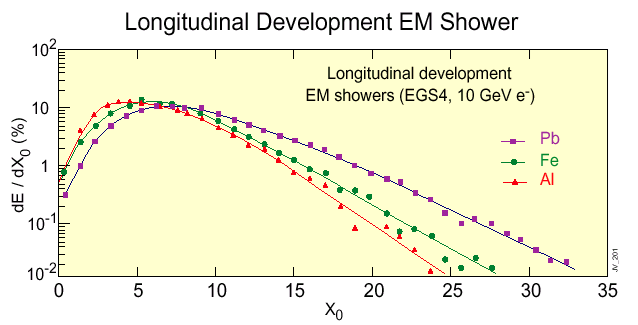
\includegraphics[width=0.7\textwidth]{immagini/grafico_longitudinale.png}
\end{figure}

Guardando lo sviluppo dello sciame da un punto di vista longitudinale abbiamo un grafico come quello che vediamo in figura sopra, in cui possiamo vedere delle simulazioni effettuate nel caso di sciami elettromagnetici prodotti da elettroni di 10 GeV. Se andiamo a vedere la perdita di energia per unità di lunghezza di radiazione (espressa qui in percentuale) ci rendiamo conto che l'energia non viene persa tutta quanta fino a quando non si raggiunge un massimo, ma in realtà ci sono delle perdite di energia anche a distanze notevoli, quindi le particelle che compongono lo sciame continuano a depositare energia nel materiale anche parecchio oltre il massimo. Notiamo come il fatto di esprimere la perdita di energia in unità di lunghezza di radiazione ci permette di confrontare facilmente materiali con densità molto diverse.

Andando a guardare le percentuali, si può dire che grosso modo il 95\% di uno sciame è contenuto longitudinalmente entro venti lunghezze di radiazione, quindi spesso quando si progettano dei calorimetri la scelta che si fa per stabilirne lo spessore è quella di scegliere una lunghezza pari a $20X_0$, in modo da essere sicuri che praticamente il 95\% dello sciame (e quindi della sua energia) sia stato depositato nel rivelatore.

\subsection{Sviluppo laterale di uno sciame e.m.}
Lo sciame non si sviluppa solo longitudinalmente, bensì ha anche una sua dimensione trasversale o laterale. Infatti, tornando di nuovo allo schema semplificato, vediamo come, a causa di diversi meccanismi (ad esempio l'angolo di apertura nella coppia $e^+ - e^-$ oppure l'angolo a cui sono emessi i fotoni di frenamento), le particelle man mano non seguiranno più la stessa direzione della particella incidente ma cominceranno ad avere direzioni diverse. La conseguenza è che lo sciame avrà una sua larghezza lateralmente, cioè nella direzione trasversale alla direzione longitudinale.

Possiamo andare a valutare le dimensioni laterali di uno sciame. Stavolta però non lavoreremo più in termini di lunghezza di radiazione, in quanto l'allargamento trasversale è descritto dal cosiddetto \textit{raggio di Molière}, che è un altro parametro legato alle proprietà del materiale utilizzato. Esso può essere approssimato dalla legge
\begin{equation*}
    R_{M}=0.0265 X_0 (Z + 1.2)
\end{equation*}
e quindi dipende dalla lunghezza di radiazione ma anche dallo $Z$ del materiale.

Ci chiediamo ora che dimensioni debba avere un cilindro in grado di contenere il 95\% dello sciame. Abbiamo visto che questo cilindro avrà altezza pari all'incirca a 20 lunghezze di radiazione, mentre in termini laterali o trasversali possiamo andare a vedere quanti raggi di Molière sono necessari per andare a contenere il 95\% dello sciame. In questo caso basta andare a considerare una dimensione pari a $2R_M$.

\begin{figure}[H]
    \centering
    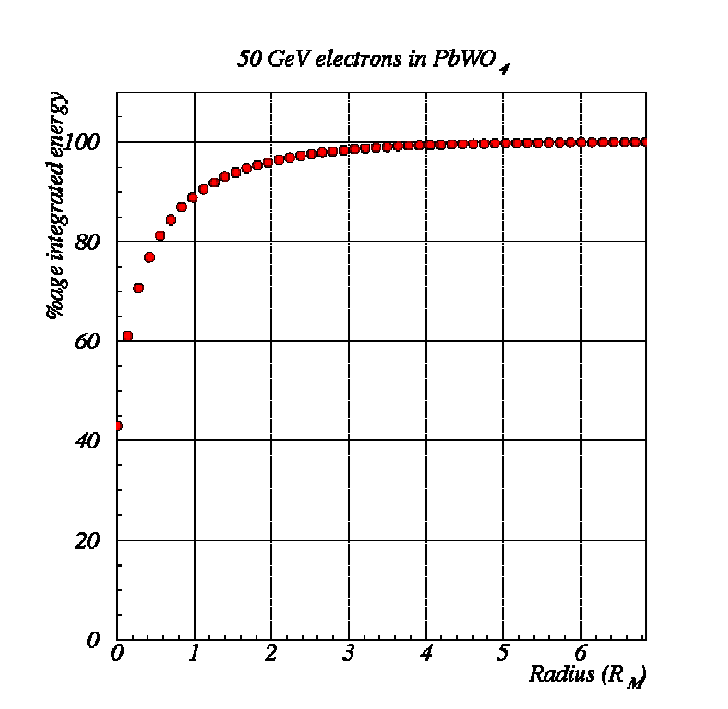
\includegraphics[width=0.52\textwidth]{immagini/raggio_di_Moliere_1.png}
\end{figure}

Infatti se andiamo a vedere quant'è la percentuale di energia che viene depositata all'interno di un materiale in funzione di $R_M$, se ci manteniamo a valori di frazioni del raggio di Molière, l'energia che possiamo ricostruire dunque l'energia che viene effettivamente depositata nel materiale sarà soltanto una frazione, intorno a $40\%-60\%$. Chiaramente, man mano che allarghiamo la base di questo cilindro andiamo a includere sempre più particelle dello sciame, quindi andiamo a considerare la quasi totalità dell'energia dello sciame. Infatti nel grafico vediamo che questa percentuale cumulativa tende a salire fino a raggiungere il 100\%. Ad esempio se ci fermiamo a $2R_M$ arriviamo appunto ad una percentuale del 95\%.

Se guardiamo un po' più nel dettaglio lo sviluppo laterale dello sciame, ci accorgiamo anche di un'altra proprietà. Guardiamo la figura seguente, in cui è rappresenta ancora la perdita di energia in funzione di multipli di $R_M$, ma stavolta le diverse curve sono ottenute per lunghezze di radiazioni diverse, nel senso che sono riportate le distribuzioni trasversali dello sciame fissato il valore di profondità, ovvero la distanza longitudinale fino a cui lo sciame è penetrato.

\begin{figure}[H]
    \centering
    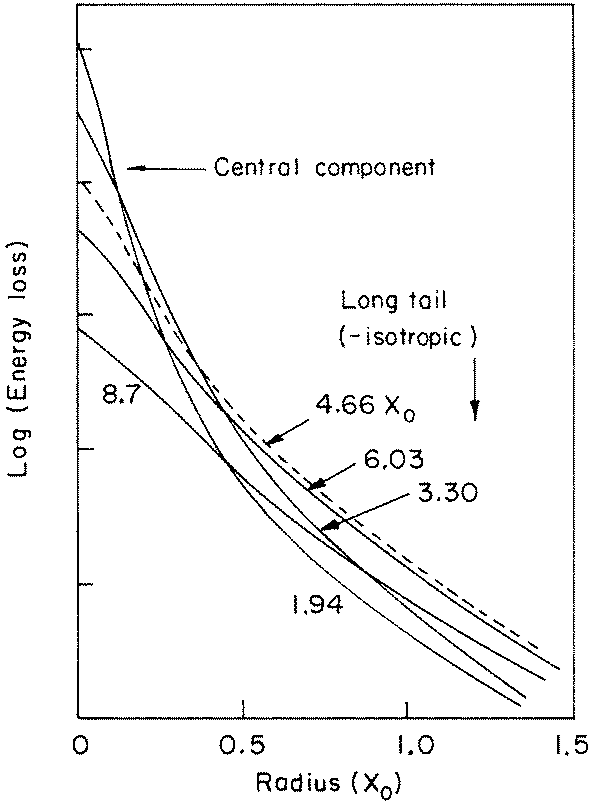
\includegraphics[width=0.4\textwidth]{immagini/raggio_di_Moliere_2.png}
\end{figure}

Notiamo come, nei casi in cui si è percorso poco spazio all'interno del materiale, la maggior parte delle particelle si concentra attorno all'asse dello sciame, cioè attorno alla direzione della particella incidente. Possiamo vedere come ad esempio la curva corrispondente a $1.94X_0$ è molto ripida ed ha un valore elevato all'inizio, il che indica che gran parte delle particelle si trova ad una distanza pari a una frazione piccola del raggio di Molière dall'asse dello sciame; ovviamente la curva man mano diminuisce, quindi ne troviamo sempre di meno a distanze maggiori dall'asse.

Man mano che lo sciame si sviluppa tende ad allargarsi, per cui se ad esempio osserviamo la curva relativa a $8,7X_0$ ci rendiamo conto che questa curva è molto diversa, infatti si ha una sorta di alone\footnote{Credo che la professoressa intenda il fatto che la curva è sostanzialmente lineare.}, quindi le particelle non si distribuiscono più in quanto hanno perso un po' l'informazione originaria della direzione della particelle incidente, per cui le ritroviamo spalmate a diverse distanze dall'asse e quindi la curva diventa nettamente meno rigida.

Quindi oltre a valutare complessivamente qual è la dimensione del raggio del cilindro che contiene il 95\% dello sciame possiamo andare a studiare un po' più nel dettaglio come sono distribuite le particelle e abbiamo visto che questo aspetto dipende dalla distanza percorsa considerata: se lo sciame è stato appena originato allora le particelle prodotte mantengono ancora un'informazione della direzione della particella incidente e dunque sono molto concentrate attorno all'asse, man mano che lo sciame si propaga nel materiale queste particelle tendono via via a cambiare direzione e quindi sono più sparpagliate, tant'è che le ritroviamo anche a distanze notevoli rispetto all'asse.

\comment{
\subsection{Simulazioni di sciami e.m.}

\textit{Questa section non so se metterla, alla fine sono solo esempi}

Vediamo adesso delle vere e proprie simulazioni\footnote{Fonte: \url{https://www.mpp.mpg.de/~menke/elss/}} verificato che ancora funziona quindi se avete voglia e piacere potete andare a vedere appunto diverse simulazioni di sciami e le trommagnetici vi faccio vedere una sequenza di sciami anche per vedere poi nel concreto tutte le proprietà che abbiamo descritta voce quindi partiamo ad esempio da questo sciame che è generato da elettroni di 8 jev in uno scintillatore di ioduro discesio non abbiamo studiato che cos'è lo scintillatore comunque vi dico semplicemente un rivelatore che andremo a studiare che dovereremo anche il laboratorio dovete immaginare che è una sorta di blocchetto di sembra un vetro sostanzialmente un vetro parecchio pesante però ha tutta l'apparenza di un materiale vetroso e quindi immaginate di avere appunto questo parallelepiped o di scintillatore e con un certo angolo di incidenza penetra un elettrone con un energia notevole vi ricordo appunto che l'energia delle sorgenti beta sono normalmente dell'ordine del med quindi probabilmente sono elettroni che sono state accelerati o prodotti da alcune reazioni e vedete cosa produce quindi questo programma non solo permette man mano di simulare l'evoluzione di uno sciame quindi simulare con tutte le sezioni di urto note i diversi meccanismi con cui può interagire prima l'elettrone e poi sui prodotti secondari ma inoltre segue il percorso di tutte le particelle prodotte le rappresentano con colori diversi ora non mi chiedete ovviamente ogni colora quale particella corrisponde però sostanzialmente troverete penso al massimo tre colori diversi che indicano appunto elettroni positroni ed elettroni positroni e fotoni e quindi vedete appunto come della particella incidente quello in giallo dovrebbe essere lasse quindi la direzione iniziale poi si genera uno sciame di particelle estremamente complicato che inizialmente aumentere il numero poi riuscire a giurto punto incominciano a degredarsi perché vengono assorbite del materiale la cosa interessante è vedere lo sviluppo dello sciame quindi vedete ha una sua lunghezza in questo caso la maggior parte dei prodotti rimane all'interno del rivelatore capite che se una di queste particelle fuoriesce è una particella che non depositerà la sua energia nel rivelatore e quindi io perdo l'informazione sulla energia cioè parte dell'energia viene persa non riesco a ricostruire l'energia di partenza del fotone quindi la mia bravura deve stare nel costruire il rivelatore sufficientemente grande da contenere gli sciami che si possono innescare all'interno chiaramente le dimensioni dello sciame l'abbiamo visto dipendono dalle energie in gioco più e grande dell'energia più grande lo sciame sia in termini nongitudinali che transversali e tuttavia fortunatamente non abbiamo una dipendenza lineare con l'energia ma lo di ritmica e quindi vedete qui il percorso delle particelle all'interno di questo blocco di scintillatore questo è un altro esempio ad esempio elettroni da ventigèvo quindi ancora più energetici in un altro materiale in questo caso neon liquido in particolare qua vedete delle tracce curvate perché probabilmente il putte è stato disposto all'interno di un campo magnetico per curvare le particelle cariche oppure elettroni da 24 Gerv su ferro quindi anche base al tipo di materiale capite che cambia la forma dello sciame cambia la sua profondità e cambia la sua larghezza transversale quindi è fondamentale andare a definire le dimensioni dello sciame conoscendo la lunghezza di radiazione e il raggio di Molière questa è una simulazione per vedere appunto dei $\gamma$ in questo caso da 5 Gerv su ferro lo vedete appunto riuscito a vedere l'animazione vero? Sì sì sì ok io regardiamo la differenza all'aumentare dell'energia questo ad esempio sono elettroni da un Gerv su uno scintillatore di vetra pionbo comunque non mi interessa il materiale specifico è al solito uno scintillatore andiamo a guardare un po' l'evoluzione di questo sciame quindi abbiamo la particella incitente e poi vedete appunto che si generano un certo numero di particelle secondare e qui abbiamo elettroni da un Gerv elettroni da due Gerv già vediamo come aumenta la profondità dello sciame e anche la sua larghezza 5 Gerv vi faccio vedere una cosa vi faccio notare una cosa oltre appunto a questo aspetto sulla dimensione transversale e longitudinale vi volevo far vedere anche che il punto di interazione del $\gamma$ cambia non avviene l'interazione sempre scusate del $\gamma$ dell'elettrone l'interazione non avviene sempre nello stesso punto e questo deriva dal fatto che abbiamo una certa probabilità una certa sezione d'urto di interazione sia di elettroni che di $\gamma$ quindi ad esempio il primo punto di nesco diciamo di questo sciame non è sempre lo stesso perché dipende appunto da questa sezione d'urto comunque sia vedete che un po' tutti i prodotti del di questo sciame si mantengono all'interno di questo scintillatore passiamo a elettroni a 10 Gerv vedete come il numero di particelle aumenta notevolmente anche la sua profondità e 20 Gerv mi ricordo se c'è altro dopo si 40 Gerv vedete che il numero di particelle è notevolmente più elevato abbiamo anche gli ottontagevano ricordavo il numero di particelle se ricordate dipende dall'energia iniziale
}